% Created by tikzDevice version 0.12.5 on 2023-10-23 23:03:40
% !TEX encoding = UTF-8 Unicode
\definecolor{color1}{HTML}{CC9966}
\definecolor{color2}{HTML}{99CCFF}
\definecolor{color3}{HTML}{77DD77}

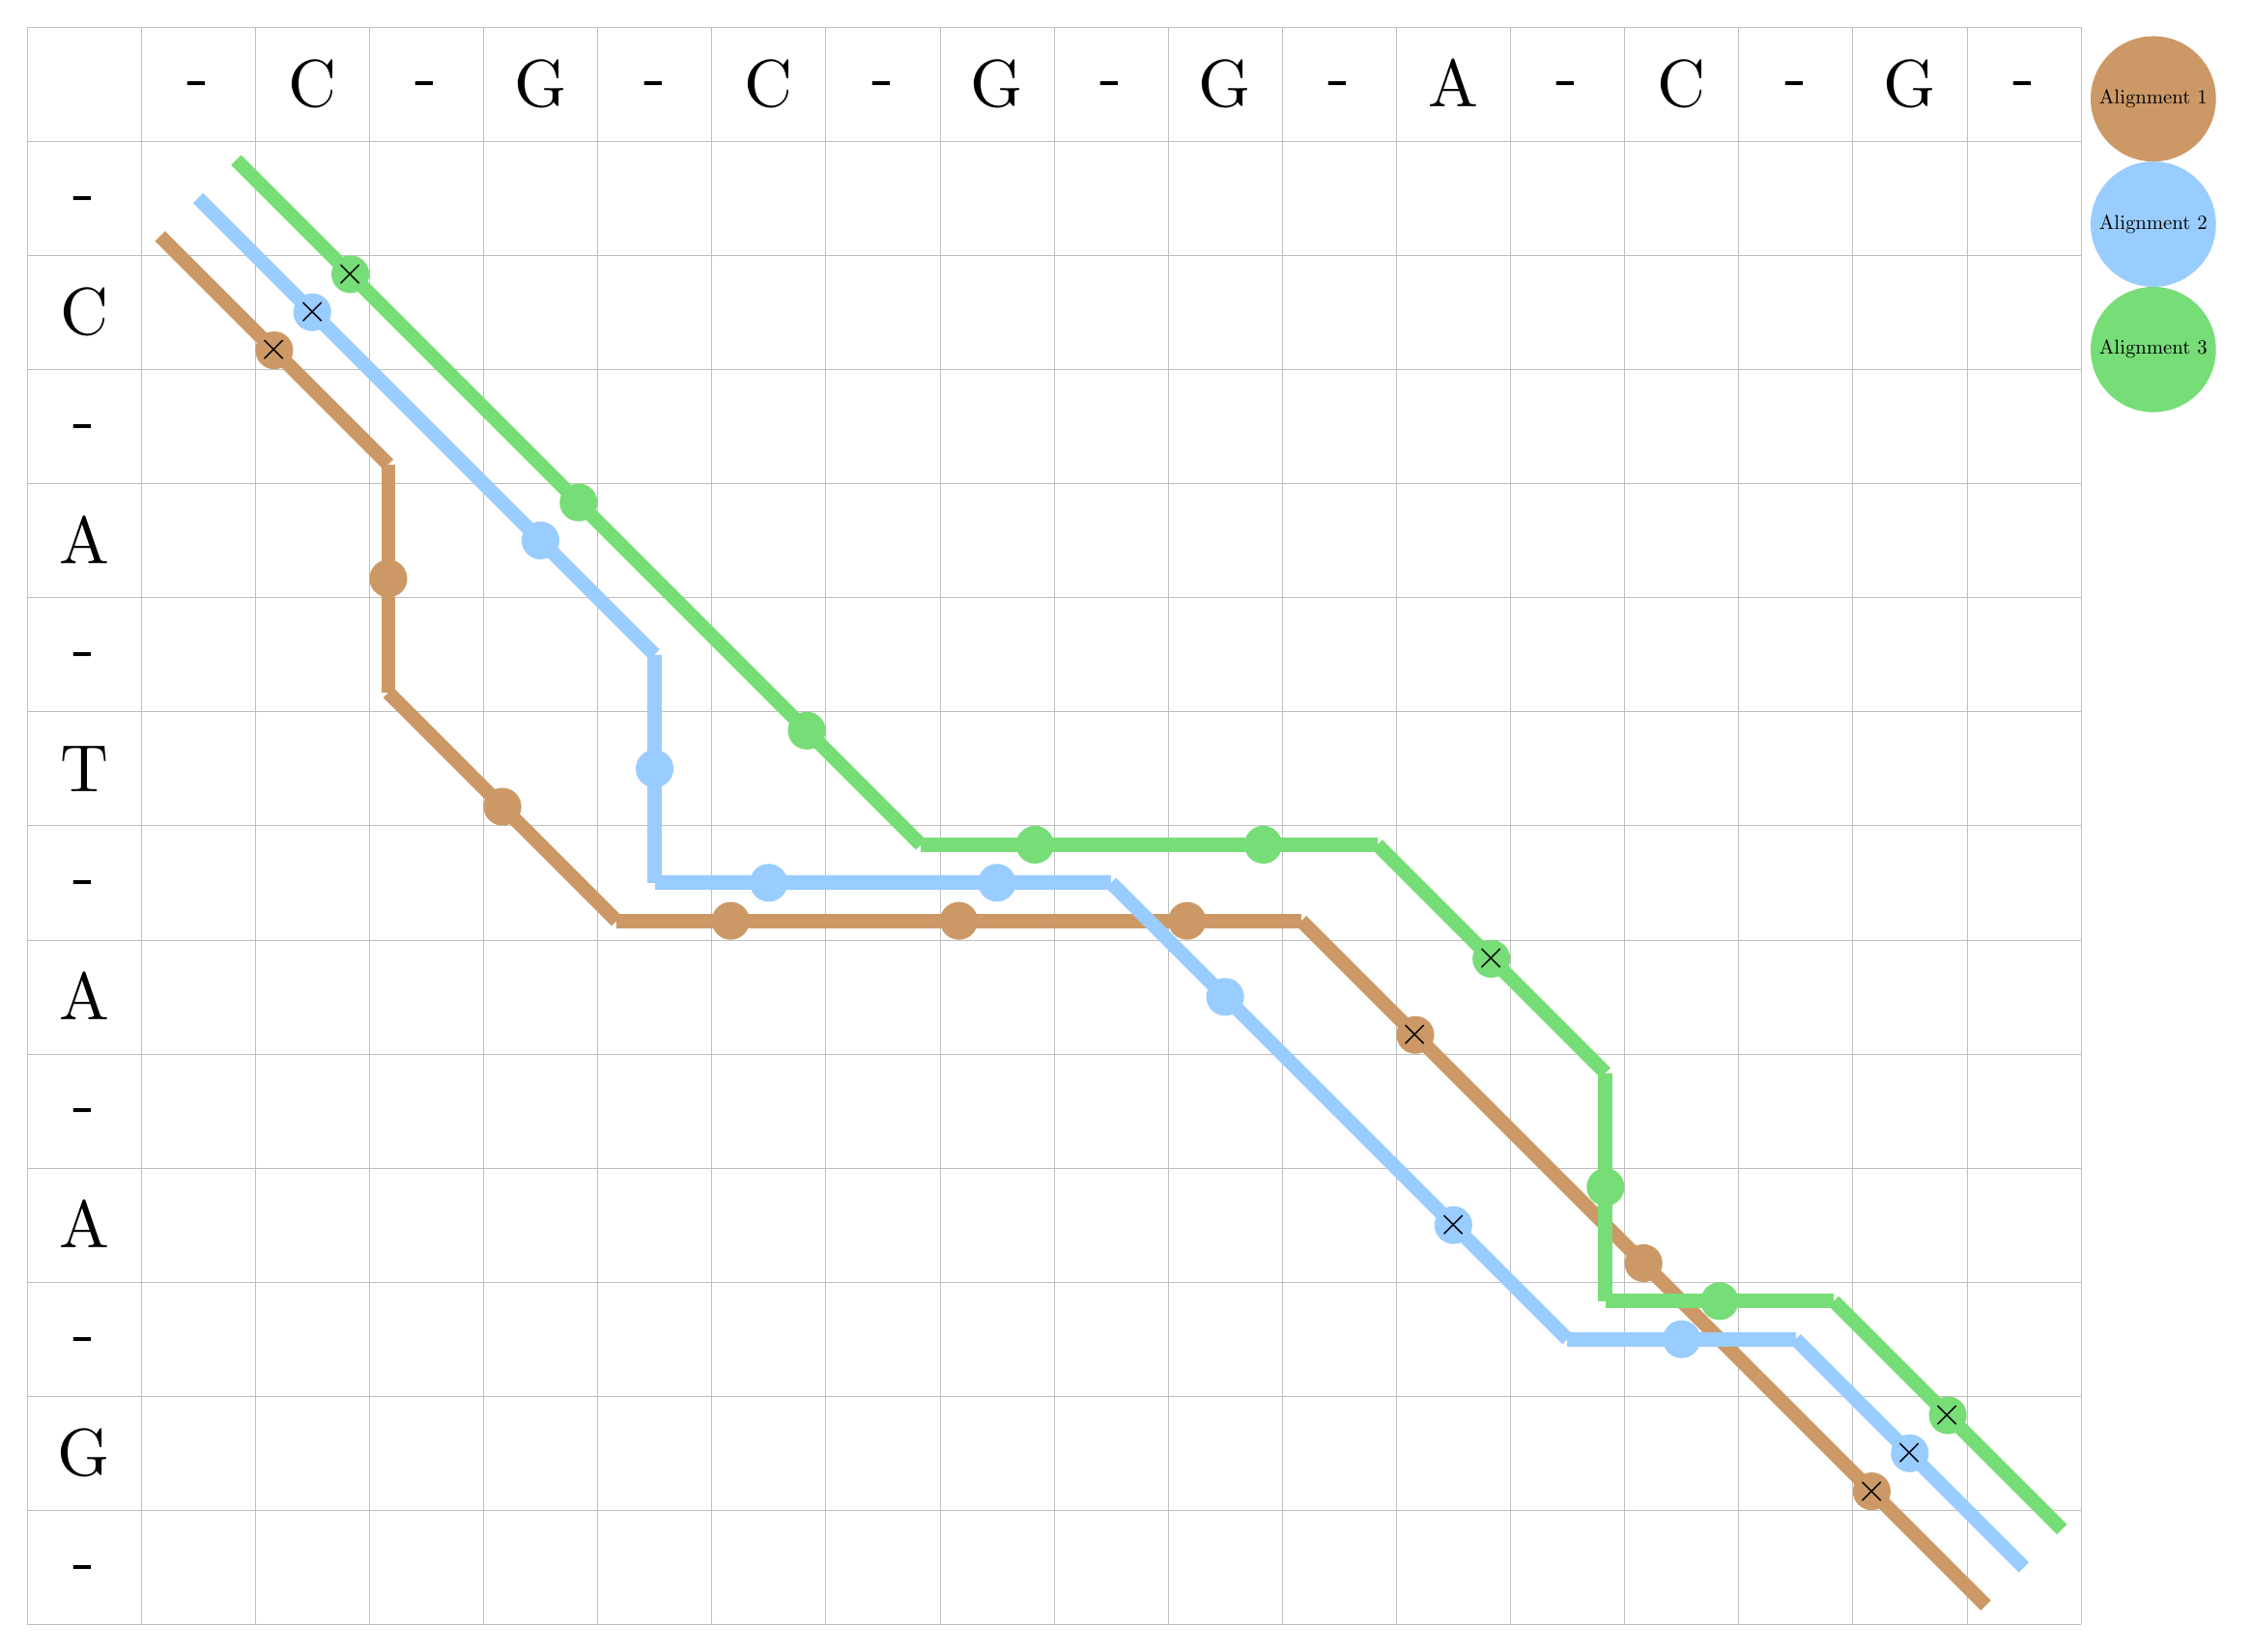
\begin{tikzpicture}[dot/.style={circle,scale=1.5, minimum size=1cm, inner sep=0pt, outer sep=0pt}]
\draw[very thin, color = gray!50, step = 1.5] (0,0) grid (27, 21);
\node [scale=2.5] at (0.75,18.75) {-};
\node [scale=2.5] at (0.75,17.25) {C};
\node [scale=2.5] at (0.75,15.75) {-};
\node [scale=2.5] at (0.75,14.25) {A};
\node [scale=2.5] at (0.75,12.75) {-};
\node [scale=2.5] at (0.75,11.25) {T};
\node [scale=2.5] at (0.75,9.75) {-};
\node [scale=2.5] at (0.75,8.25) {A};
\node [scale=2.5] at (0.75,6.75) {-};
\node [scale=2.5] at (0.75,5.25) {A};
\node [scale=2.5] at (0.75,3.75) {-};
\node [scale=2.5] at (0.75,2.25) {G};
\node [scale=2.5] at (0.75,0.75) {-};
\node [scale=2.5] at (2.25,20.25) {-};
\node [scale=2.5] at (3.75,20.25) {C};
\node [scale=2.5] at (5.25,20.25) {-};
\node [scale=2.5] at (6.75,20.25) {G};
\node [scale=2.5] at (8.25,20.25) {-};
\node [scale=2.5] at (9.75,20.25) {C};
\node [scale=2.5] at (11.25,20.25) {-};
\node [scale=2.5] at (12.75,20.25) {G};
\node [scale=2.5] at (14.25,20.25) {-};
\node [scale=2.5] at (15.75,20.25) {G};
\node [scale=2.5] at (17.25,20.25) {-};
\node [scale=2.5] at (18.75,20.25) {A};
\node [scale=2.5] at (20.25,20.25) {-};
\node [scale=2.5] at (21.75,20.25) {C};
\node [scale=2.5] at (23.25,20.25) {-};
\node [scale=2.5] at (24.75,20.25) {G};
\node [scale=2.5] at (26.25,20.25) {-};
\draw[line width=1.875mm,color1](1.75,18.25)--(3.25,16.75);
\draw[line width=1.875mm,color1](3.25,16.75)--(4.75,15.25);
\node[circle,scale=1.5, fill=color1] at (3.25, 16.75){};
\node[black,scale=1.5] at (3.25, 16.75){$\mathlarger{\mathlarger{\bm{\times}}}$};
\draw[line width=1.875mm,color1](4.75,15.25)--(4.75,13.75);
\draw[line width=1.875mm,color1](4.75,13.75)--(4.75,12.25);
\node[circle,scale=1.5, fill=color1] at (4.75, 13.75){};
\draw[line width=1.875mm,color1](4.75,12.25)--(6.25,10.75);
\draw[line width=1.875mm,color1](6.25,10.75)--(7.75,9.25);
\node[circle,scale=1.5, fill=color1] at (6.25, 10.75){};
\draw[line width=1.875mm,color1](7.75,9.25)--(9.25,9.25);
\draw[line width=1.875mm,color1](9.25,9.25)--(10.75,9.25);
\node[circle,scale=1.5, fill=color1] at (9.25, 9.25){};
\draw[line width=1.875mm,color1](10.75,9.25)--(12.25,9.25);
\draw[line width=1.875mm,color1](12.25,9.25)--(13.75,9.25);
\node[circle,scale=1.5, fill=color1] at (12.25, 9.25){};
\draw[line width=1.875mm,color1](13.75,9.25)--(15.25,9.25);
\draw[line width=1.875mm,color1](15.25,9.25)--(16.75,9.25);
\node[circle,scale=1.5, fill=color1] at (15.25, 9.25){};
\draw[line width=1.875mm,color1](16.75,9.25)--(18.25,7.75);
\draw[line width=1.875mm,color1](18.25,7.75)--(19.75,6.25);
\node[circle,scale=1.5, fill=color1] at (18.25, 7.75){};
\node[black,scale=1.5] at (18.25, 7.75){$\mathlarger{\mathlarger{\bm{\times}}}$};
\draw[line width=1.875mm,color1](19.75,6.25)--(21.25,4.75);
\draw[line width=1.875mm,color1](21.25,4.75)--(22.75,3.25);
\node[circle,scale=1.5, fill=color1] at (21.25, 4.75){};
\draw[line width=1.875mm,color1](22.75,3.25)--(24.25,1.75);
\draw[line width=1.875mm,color1](24.25,1.75)--(25.75,0.25);
\node[circle,scale=1.5, fill=color1] at (24.25, 1.75){};
\node[black,scale=1.5] at (24.25, 1.75){$\mathlarger{\mathlarger{\bm{\times}}}$};
\draw[line width=1.875mm,color2](2.25,18.75)--(3.75,17.25);
\draw[line width=1.875mm,color2](3.75,17.25)--(5.25,15.75);
\node[circle,scale=1.5, fill=color2] at (3.75, 17.25){};
\node[black,scale=1.5] at (3.75, 17.25){$\mathlarger{\mathlarger{\bm{\times}}}$};
\draw[line width=1.875mm,color2](5.25,15.75)--(6.75,14.25);
\draw[line width=1.875mm,color2](6.75,14.25)--(8.25,12.75);
\node[circle,scale=1.5, fill=color2] at (6.75, 14.25){};
\draw[line width=1.875mm,color2](8.25,12.75)--(8.25,11.25);
\draw[line width=1.875mm,color2](8.25,11.25)--(8.25,9.75);
\node[circle,scale=1.5, fill=color2] at (8.25, 11.25){};
\draw[line width=1.875mm,color2](8.25,9.75)--(9.75,9.75);
\draw[line width=1.875mm,color2](9.75,9.75)--(11.25,9.75);
\node[circle,scale=1.5, fill=color2] at (9.75, 9.75){};
\draw[line width=1.875mm,color2](11.25,9.75)--(12.75,9.75);
\draw[line width=1.875mm,color2](12.75,9.75)--(14.25,9.75);
\node[circle,scale=1.5, fill=color2] at (12.75, 9.75){};
\draw[line width=1.875mm,color2](14.25,9.75)--(15.75,8.25);
\draw[line width=1.875mm,color2](15.75,8.25)--(17.25,6.75);
\node[circle,scale=1.5, fill=color2] at (15.75, 8.25){};
\draw[line width=1.875mm,color2](17.25,6.75)--(18.75,5.25);
\draw[line width=1.875mm,color2](18.75,5.25)--(20.25,3.75);
\node[circle,scale=1.5, fill=color2] at (18.75, 5.25){};
\node[black,scale=1.5] at (18.75, 5.25){$\mathlarger{\mathlarger{\bm{\times}}}$};
\draw[line width=1.875mm,color2](20.25,3.75)--(21.75,3.75);
\draw[line width=1.875mm,color2](21.75,3.75)--(23.25,3.75);
\node[circle,scale=1.5, fill=color2] at (21.75, 3.75){};
\draw[line width=1.875mm,color2](23.25,3.75)--(24.75,2.25);
\draw[line width=1.875mm,color2](24.75,2.25)--(26.25,0.75);
\node[circle,scale=1.5, fill=color2] at (24.75, 2.25){};
\node[black,scale=1.5] at (24.75, 2.25){$\mathlarger{\mathlarger{\bm{\times}}}$};
\draw[line width=1.875mm,color3](2.75,19.25)--(4.25,17.75);
\draw[line width=1.875mm,color3](4.25,17.75)--(5.75,16.25);
\node[circle,scale=1.5, fill=color3] at (4.25, 17.75){};
\node[black,scale=1.5] at (4.25, 17.75){$\mathlarger{\mathlarger{\bm{\times}}}$};
\draw[line width=1.875mm,color3](5.75,16.25)--(7.25,14.75);
\draw[line width=1.875mm,color3](7.25,14.75)--(8.75,13.25);
\node[circle,scale=1.5, fill=color3] at (7.25, 14.75){};
\draw[line width=1.875mm,color3](8.75,13.25)--(10.25,11.75);
\draw[line width=1.875mm,color3](10.25,11.75)--(11.75,10.25);
\node[circle,scale=1.5, fill=color3] at (10.25, 11.75){};
\draw[line width=1.875mm,color3](11.75,10.25)--(13.25,10.25);
\draw[line width=1.875mm,color3](13.25,10.25)--(14.75,10.25);
\node[circle,scale=1.5, fill=color3] at (13.25, 10.25){};
\draw[line width=1.875mm,color3](14.75,10.25)--(16.25,10.25);
\draw[line width=1.875mm,color3](16.25,10.25)--(17.75,10.25);
\node[circle,scale=1.5, fill=color3] at (16.25, 10.25){};
\draw[line width=1.875mm,color3](17.75,10.25)--(19.25,8.75);
\draw[line width=1.875mm,color3](19.25,8.75)--(20.75,7.25);
\node[circle,scale=1.5, fill=color3] at (19.25, 8.75){};
\node[black,scale=1.5] at (19.25, 8.75){$\mathlarger{\mathlarger{\bm{\times}}}$};
\draw[line width=1.875mm,color3](20.75,7.25)--(20.75,5.75);
\draw[line width=1.875mm,color3](20.75,5.75)--(20.75,4.25);
\node[circle,scale=1.5, fill=color3] at (20.75, 5.75){};
\draw[line width=1.875mm,color3](20.75,4.25)--(22.25,4.25);
\draw[line width=1.875mm,color3](22.25,4.25)--(23.75,4.25);
\node[circle,scale=1.5, fill=color3] at (22.25, 4.25){};
\draw[line width=1.875mm,color3](23.75,4.25)--(25.25,2.75);
\draw[line width=1.875mm,color3](25.25,2.75)--(26.75,1.25);
\node[circle,scale=1.5, fill=color3] at (25.25, 2.75){};
\node[black,scale=1.5] at (25.25, 2.75){$\mathlarger{\mathlarger{\bm{\times}}}$};
\matrix [draw, below right, draw=none] at (current bounding box.north east) {
        \node[circle, fill=color1, scale=0.75] {Alignment 1}; \\
        \node[circle, fill=color2, scale=0.75] {Alignment 2}; \\
        \node[circle, fill=color3, scale=0.75] {Alignment 3}; \\
    };
\end{tikzpicture}
